\documentclass[aspectratio=169]{beamer}
\usepackage{panqueques}
\usepackage{amsmath}
\usepackage{amssymb}
\usepackage{tcolorbox}
\usepackage{physics}
\usepackage{amsmath}
\usepackage{tikz}
\usepackage{mathdots}
\usepackage{yhmath}
\usepackage{cancel}
\usepackage{color}
\usepackage{siunitx}
\usepackage{array}
\usepackage{multirow}
\usepackage{amssymb}
\usepackage{gensymb}
\usepackage{tabularx}
\usepackage{extarrows}
\usepackage{booktabs}
\usetikzlibrary{fadings}
\usetikzlibrary{patterns}
\usetikzlibrary{shadows.blur}
\usetikzlibrary{shapes}



\usepackage{physics}
\usepackage{amsmath}
\usepackage{tikz}
\usepackage{mathdots}
\usepackage{yhmath}
\usepackage{cancel}
\usepackage{color}
\usepackage{siunitx}
\usepackage{array}
\usepackage{multirow}
\usepackage{amssymb}
\usepackage{gensymb}
\usepackage{tabularx}
\usepackage{extarrows}
\usepackage{booktabs}
\usetikzlibrary{fadings}
\usetikzlibrary{patterns}
\usetikzlibrary{shadows.blur}
\usetikzlibrary{shapes}
\usepackage{caption}
\title{Project Report for MA4207}
\author{name}
\date{\today}

\begin{document}

%title-page %%edit in 1-title-page folder
\begin{frame}[noframenumbering,plain]
    \begin{tikzpicture}[remember picture, overlay]
        \fill[white] (current page.south west) rectangle ([xshift=4cm]current page.north west);
        \node at ([xshift=2cm,yshift=-4.5cm]current page.north west) {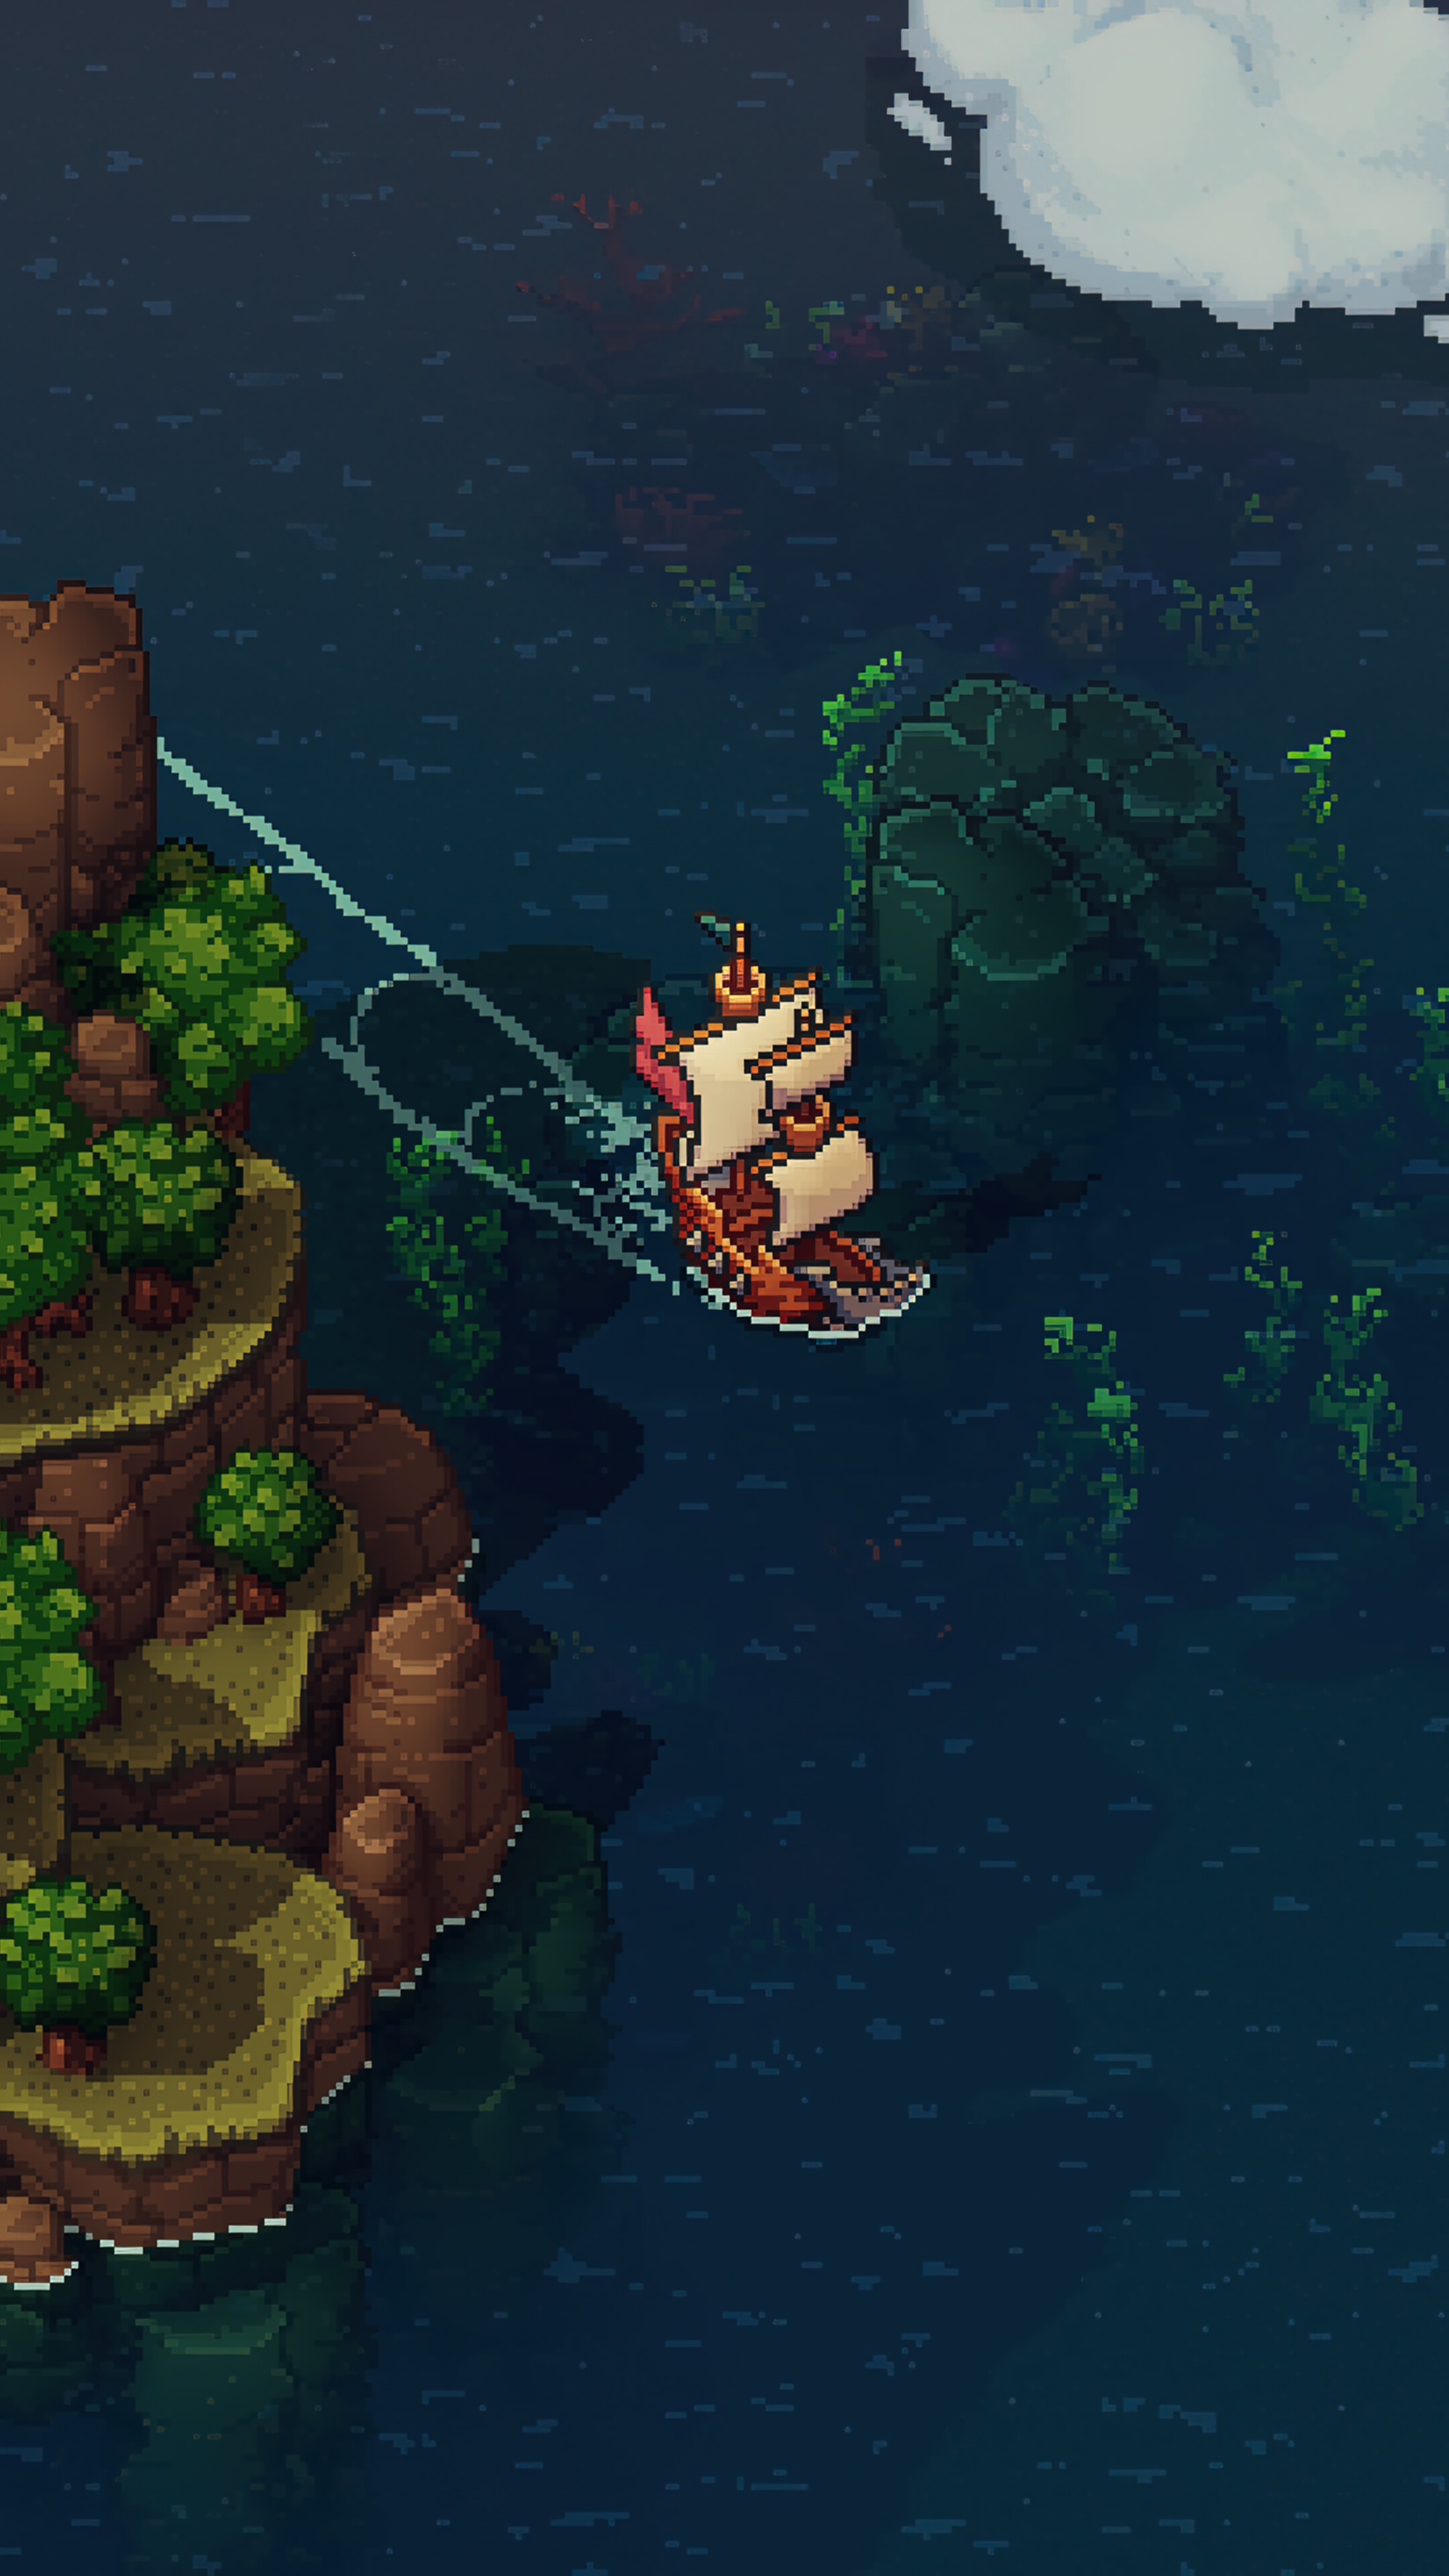
\includegraphics[width=9cm]{1-title-page/cover.jpg}};
    \end{tikzpicture}
    \begingroup  
        \flushright
        {\fontfamily{qag}\selectfont\Huge\bfseries\color{black}Stationary\\ Information\\ Sources}\vspace{1em}\\
        Aakash Ghosh\vspace{0.5em}\\
        \MyDate\par
    \endgroup
\end{frame}

%edit as needed

%content %%edit in 2-content -> content.tex
%introduction-example








\begin{frame}{Timeline}    
   We shall look at the following:\\
   \textbf{1.} Prediction of earthquake\pause\\
   \textbf{2.} Classification of EEG data\pause\\
   \textbf{3.} Network analysis
\end{frame}



\begin{frame}{Earthquake Prediction-Problem Description}
We look at the problem description:
    \begin{enumerate}[$\bullet$]
        \item \textbf{Problem}: Predicting whether a major earthquake event is about to occur based on recent readings in the surrounding area\pause
        \item \textbf{Task}: Binary classification\pause
        \item \textbf{Positive case}: A major event (reading over 5 on the Rictor scale) not preceded by another major event for at least 512 hours\pause
        \item \textbf{Negative case}: A reading below 4 that is preceded by at least 20 readings in the previous 512 hours that are non-zero\pause
        \item \textbf{Goal}: Accurately classify each instance as a positive or negative case to improve earthquake prediction and preparation efforts.
    \end{enumerate}
\end{frame}




\begin{frame}{Looking for patterns}
    \begin{columns}[T]
    \begin{column}{0.4\textwidth}
      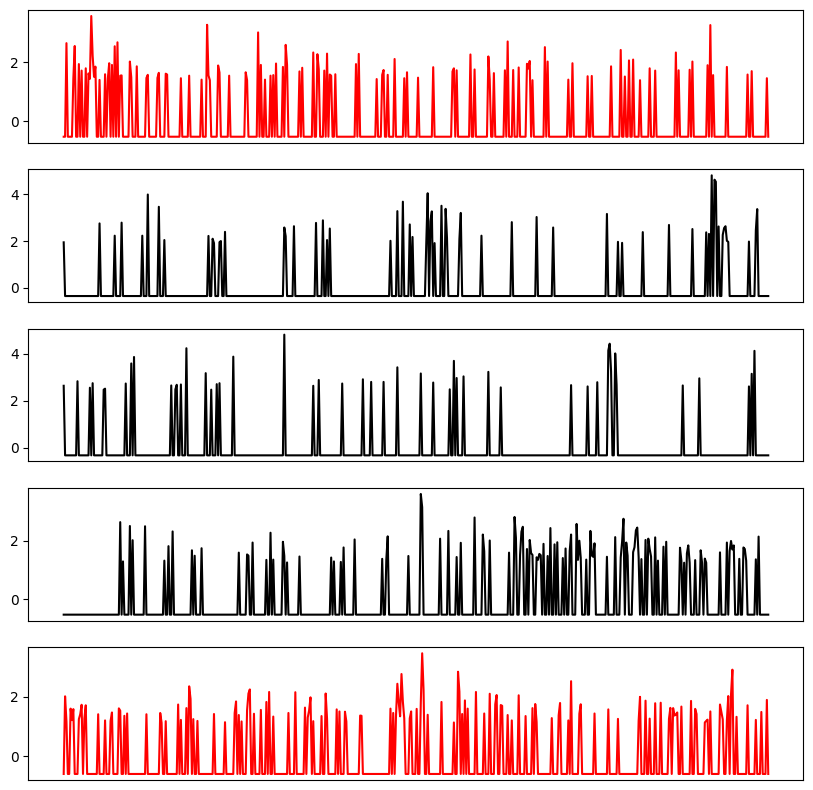
\includegraphics[width=\textwidth]{images/TSP.png}
    \end{column}
    \begin{column}{0.6\textwidth}
    \begin{enumerate}[$\bullet$]
    \item The first 5 rows of the time series data were plotted, with positive cases highlighted in red and negative cases in black.\pause
    \item Upon visual inspection, we observed that positive cases had a higher number of peaks compared to negative cases.\pause 
    \item This observation motivated us to use the bag of words approach to capture the shapes of these peaks as potential features for our classifier.
    \end{enumerate}
    \end{column}
  \end{columns}
\end{frame}

\begin{frame}{Bag of Words approach}
    \begin{columns}[T]
    \begin{column}{0.8\textwidth}
    Bag of words approach is a common technique in natural language processing (NLP) for feature extraction. It represents a text document as a "bag" of its words, disregarding grammar and word order but retaining information about word frequency. This approach identifies important words that are most indicative of the document's content.\pause\\\vspace{1cm}
    We apply a similar approach to time series data instead of text data. We represent time series data as a bag of peaks, allowing us to capture information about the shapes and lengths of the peaks. This information can be used as features for our classifier.
    \end{column}
    \begin{column}{0.3\textwidth}
        

\tikzset{every picture/.style={line width=0.75pt}} %set default line width to 0.75pt        


\tikzset{every picture/.style={line width=0.75pt}} %set default line width to 0.75pt        

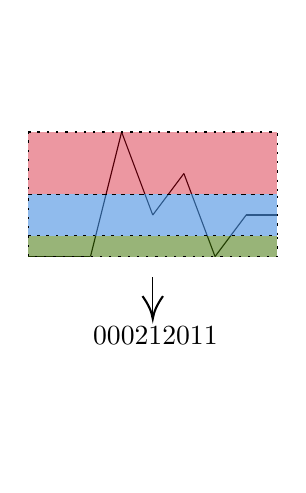
\begin{tikzpicture}[x=0.75pt,y=0.75pt,yscale=-1,xscale=1.5]
%uncomment if require: \path (0,300); %set diagram left start at 0, and has height of 300

%Straight Lines [id:da6973883485240086] 
\draw    (20,150) -- (40,150) ;
%Straight Lines [id:da4843828656242116] 
\draw    (40,150) -- (50,90) ;
%Straight Lines [id:da5387802093437941] 
\draw    (50,90) -- (60,130) ;
%Straight Lines [id:da9438003440894683] 
\draw    (60,130) -- (70,110) ;
%Straight Lines [id:da2525091782720156] 
\draw    (70,110) -- (80,150) ;
%Straight Lines [id:da303722386805403] 
\draw    (80,150) -- (90,130) ;
%Straight Lines [id:da026393717543859996] 
\draw    (90,130) -- (100,130) ;
%Straight Lines [id:da5167510940637614] 
\draw  [dash pattern={on 0.84pt off 2.51pt}]  (20,140) -- (100,140) ;
%Straight Lines [id:da8942416198464498] 
\draw  [dash pattern={on 0.84pt off 2.51pt}]  (20,120) -- (100,120) ;
%Straight Lines [id:da28363237003689823] 
\draw    (60,160) -- (60,178) ;
\draw [shift={(60,180)}, rotate = 270] [color={rgb, 255:red, 0; green, 0; blue, 0 }  ][line width=0.75]    (10.93,-3.29) .. controls (6.95,-1.4) and (3.31,-0.3) .. (0,0) .. controls (3.31,0.3) and (6.95,1.4) .. (10.93,3.29)   ;
%Shape: Rectangle [id:dp7253302883790628] 
\draw  [color={rgb, 255:red, 0; green, 0; blue, 0 }  ,draw opacity=1 ][fill={rgb, 255:red, 74; green, 144; blue, 226 }  ,fill opacity=0.61 ][dash pattern={on 0.84pt off 2.51pt}] (20,120) -- (100,120) -- (100,140) -- (20,140) -- cycle ;
%Shape: Rectangle [id:dp0036813331224995194] 
\draw  [fill={rgb, 255:red, 65; green, 117; blue, 5 }  ,fill opacity=0.54 ][dash pattern={on 0.84pt off 2.51pt}] (20,140) -- (100,140) -- (100,150) -- (20,150) -- cycle ;
%Shape: Rectangle [id:dp4949784549292484] 
\draw  [fill={rgb, 255:red, 208; green, 2; blue, 27 }  ,fill opacity=0.41 ][dash pattern={on 0.84pt off 2.51pt}] (20,90) -- (100,90) -- (100,120) -- (20,120) -- cycle ;
%Shape: Rectangle [id:dp5751895584090528] 
\draw  [draw opacity=0] (20,40) -- (100,40) -- (100,250) -- (20,250) -- cycle ;

% Text Node
\draw (40,182.4) node [anchor=north west][inner sep=0.75pt]    {$000212011$};


\end{tikzpicture}

    \end{column}
  \end{columns}
\end{frame}


\begin{frame}{Bag of words approach(contd.)}
\begin{columns}[T]
    \begin{column}{0.6\textwidth}
      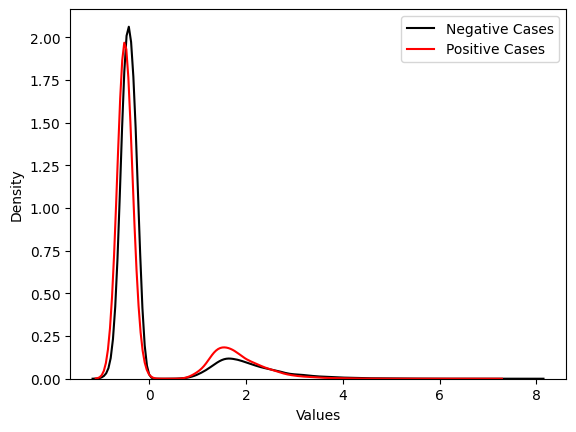
\includegraphics[width=\textwidth]{images/density.png}
    \end{column}
    \begin{column}{0.45\textwidth}
    We analyze the density distribution of the distinct classes, i.e., positive and negative cases. To apply the BoW approach, we assign each demarcating interval a letter. We can then generate words of length 4 using these letters to capture important information about the shapes of the peaks. We extract those words using a moving window.
    \end{column}
  \end{columns}
\end{frame}

\begin{frame}{Bag of words approach(contd.)}
    \begin{figure}
        \centering
\tikzset{every picture/.style={line width=0.75pt}} %set default line width to 0.75pt        

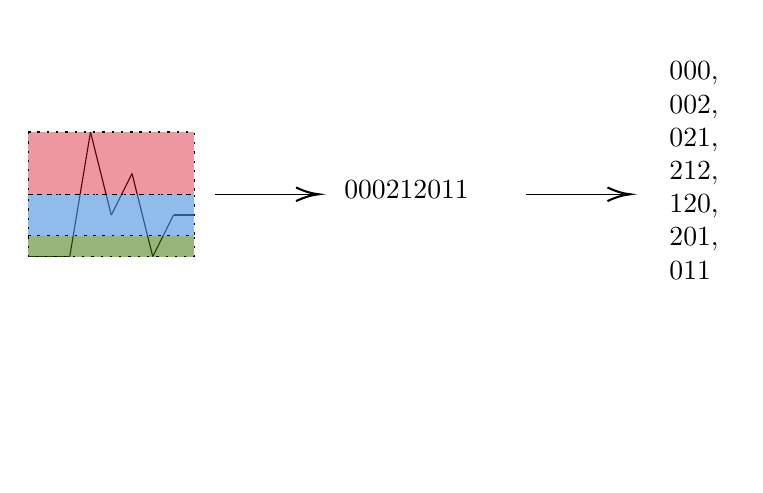
\begin{tikzpicture}[x=0.75pt,y=0.75pt,yscale=-1,xscale=1]
%uncomment if require: \path (0,300); %set diagram left start at 0, and has height of 300

%Straight Lines [id:da6973883485240086] 
\draw    (20,150) -- (40,150) ;
%Straight Lines [id:da4843828656242116] 
\draw    (40,150) -- (50,90) ;
%Straight Lines [id:da5387802093437941] 
\draw    (50,90) -- (60,130) ;
%Straight Lines [id:da9438003440894683] 
\draw    (60,130) -- (70,110) ;
%Straight Lines [id:da2525091782720156] 
\draw    (70,110) -- (80,150) ;
%Straight Lines [id:da303722386805403] 
\draw    (80,150) -- (90,130) ;
%Straight Lines [id:da026393717543859996] 
\draw    (90,130) -- (100,130) ;
%Straight Lines [id:da5167510940637614] 
\draw  [dash pattern={on 0.84pt off 2.51pt}]  (20,140) -- (100,140) ;
%Straight Lines [id:da8942416198464498] 
\draw  [dash pattern={on 0.84pt off 2.51pt}]  (20,120) -- (100,120) ;
%Straight Lines [id:da28363237003689823] 
\draw    (110,120) -- (158,120) ;
\draw [shift={(160,120)}, rotate = 180] [color={rgb, 255:red, 0; green, 0; blue, 0 }  ][line width=0.75]    (10.93,-3.29) .. controls (6.95,-1.4) and (3.31,-0.3) .. (0,0) .. controls (3.31,0.3) and (6.95,1.4) .. (10.93,3.29)   ;
%Shape: Rectangle [id:dp7253302883790628] 
\draw  [color={rgb, 255:red, 0; green, 0; blue, 0 }  ,draw opacity=1 ][fill={rgb, 255:red, 74; green, 144; blue, 226 }  ,fill opacity=0.61 ][dash pattern={on 0.84pt off 2.51pt}] (20,120) -- (100,120) -- (100,140) -- (20,140) -- cycle ;
%Shape: Rectangle [id:dp0036813331224995194] 
\draw  [fill={rgb, 255:red, 65; green, 117; blue, 5 }  ,fill opacity=0.54 ][dash pattern={on 0.84pt off 2.51pt}] (20,140) -- (100,140) -- (100,150) -- (20,150) -- cycle ;
%Shape: Rectangle [id:dp4949784549292484] 
\draw  [fill={rgb, 255:red, 208; green, 2; blue, 27 }  ,fill opacity=0.41 ][dash pattern={on 0.84pt off 2.51pt}] (20,90) -- (100,90) -- (100,120) -- (20,120) -- cycle ;
%Shape: Rectangle [id:dp5751895584090528] 
\draw  [draw opacity=0] (20,40) -- (100,40) -- (100,250) -- (20,250) -- cycle ;
%Straight Lines [id:da759026028696174] 
\draw    (260,120) -- (308,120) ;
\draw [shift={(310,120)}, rotate = 180] [color={rgb, 255:red, 0; green, 0; blue, 0 }  ][line width=0.75]    (10.93,-3.29) .. controls (6.95,-1.4) and (3.31,-0.3) .. (0,0) .. controls (3.31,0.3) and (6.95,1.4) .. (10.93,3.29)   ;

% Text Node
\draw (171,112.4) node [anchor=north west][inner sep=0.75pt]    {$000212011$};
% Text Node
\draw (321,52.4) node [anchor=north west][inner sep=0.75pt]    {$ \begin{array}{l}
000,\\
002,\\
021,\\
212,\\
120,\\
201,\\
011
\end{array}$};


\end{tikzpicture}
    \caption*{Example of word extraction from a moving window. Words of length 3 is extracted in this case}
        \label{fig:my_label}
    \end{figure}
\end{frame}

\begin{frame}{Training}
    We shall use random forest methods because:
    \begin{enumerate}[$\bullet$]
    \item The dataset has a large number of features\pause
    \item The relationship between the features and labels may not be linear\pause
    \item Some features may not be important for the classification task
\end{enumerate}
\end{frame}

\begin{frame}{Training(contd.)}
   \begin{columns}[T]
    \begin{column}{0.6\textwidth}
      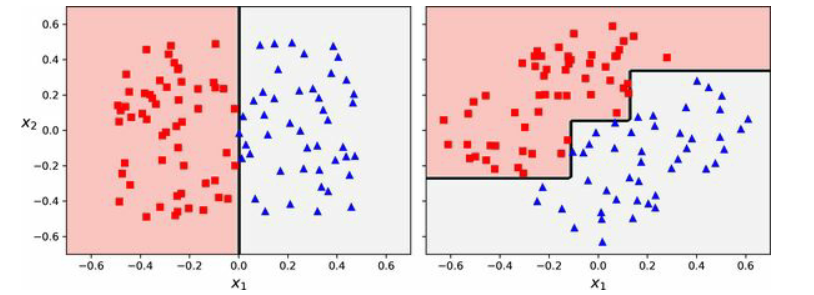
\includegraphics[width=1\textwidth]{images/PCA_for_RF.png}
    \end{column}
    \begin{column}{0.4\textwidth}
    Random tree classifiers draw decision boundaries parallel to the axes. However, in order to improve the decision boundaries by maximizing variance across each axis, we can apply PCA (Principal Component Analysis) to increase the variance across each axis.
    \end{column}
  \end{columns}
\end{frame}
\begin{frame}{Cross validation and Results}
We use 10-fold cross validation. The results are:
\begin{enumerate}[$\bullet$]
    \item \textbf{Mean CV score: 0.8198863636363637}\pause
    \item \textbf{CV score std: 0.0587866096395338}\pause
\end{enumerate}
We test against the test data set. We check the accuracy and the confusion matrix.
\begin{enumerate}[$\bullet$]
    \item We great an accuracy of \textbf{0.7482014388489209}\pause
    \item The confusion matrix is:
    \begin{align*}
    \begin{bmatrix}
    101&3\\
    32&3
    \end{bmatrix}
    \end{align*}
 \end{enumerate}
\end{frame}


\begin{frame}{Motor Imagery- Problem Description}
    We look at the problem description:
    \begin{enumerate}[$\bullet$]
        \item \textbf{Problem:} The dataset consists of recordings of imagined movements of either the left small finger or the tongue using an 8x8 ECoG platinum electrode grid. The data was recorded at a sampling rate of 1000Hz, starting 0.5 seconds after the visual cue had ended and lasting for 3 seconds (series length 3000). The dataset contains 64 dimensions, representing the 8x8 electrode grid.\pause
        \item \textbf{Task:} Binary Classification\pause
        \item \textbf{Case 1:}The left small finger is moved\pause
        \item  \textbf{Case 2:}The tongue is moved
    \end{enumerate}
\end{frame}
\begin{frame}{Preprocessing}
    \begin{columns}[T]
    \begin{column}{0.6\textwidth}
      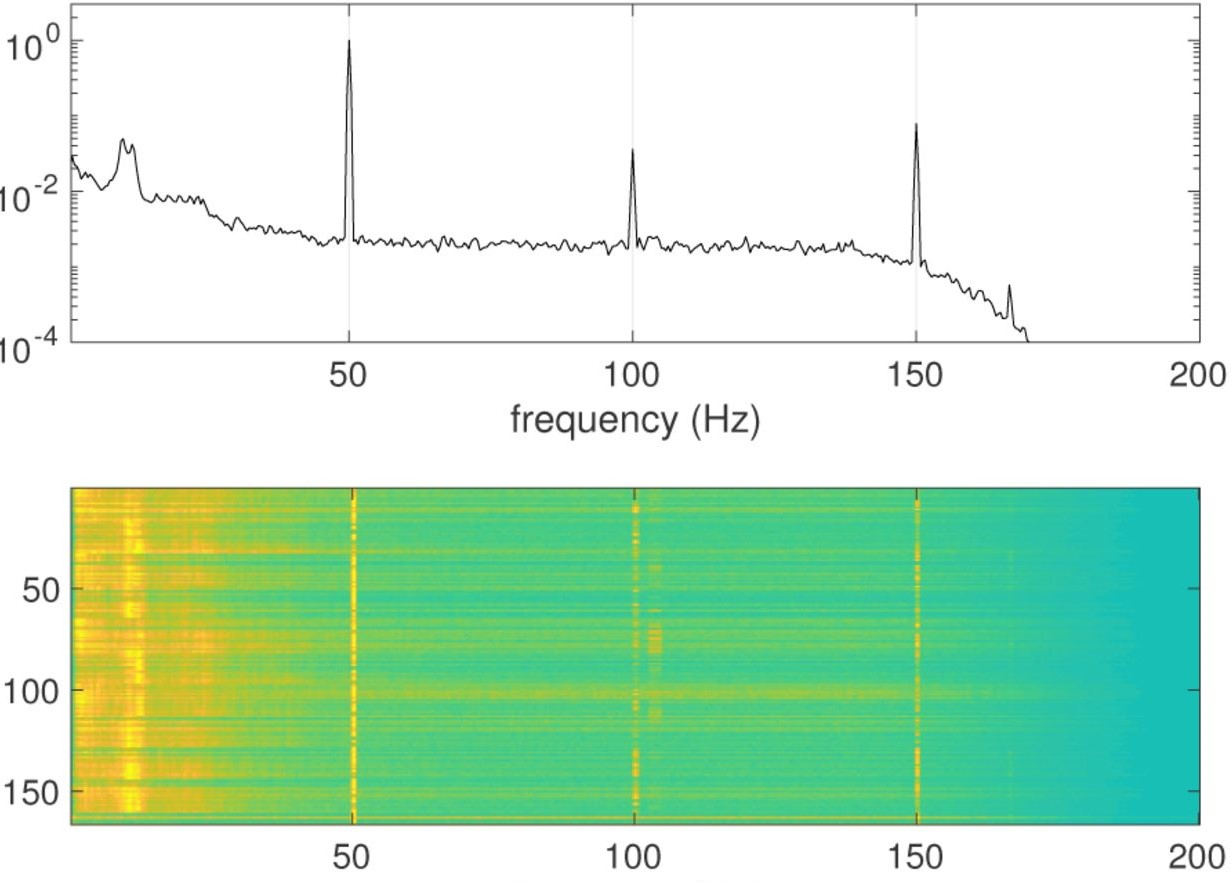
\includegraphics[width=\textwidth]{images/line.jpg}
    \end{column}
    \begin{column}{0.45\textwidth}
    Line noise is unwanted electrical signals in EEG recordings, generated from sources like power lines or electronic devices. It can cause distortion or artifact in the data and affect accuracy.\pause To improve signal-to-noise ratio and reduce artifacts, line noise removal is important in EEG preprocessing. A low-pass filter with a 45Hz threshold is used to remove noise frequencies. Removing line noise helps obtain more reliable measurements of brain activity.
    \end{column}
  \end{columns}
\end{frame}
\begin{frame}{Feature Extraction}
    We shall consider the data to be non-parametric. Non parametric time series analysis methods do not require a specific functional form for the data and are therefore more flexible than traditional parametric approaches, which often assume normality or other distributions.This leads to greater universality while trading off for little accuracy.\pause

    We shall use Burg's method, which is a popular method for feature extraction in time series data. It is a model-based method that uses autoregressive (AR) modeling to estimate the signal parameters. The method estimates the coefficients of an AR model which can then be used as features to represent the time series data.
\end{frame}

\begin{frame}{Training and Cross validation}
We use Random forest as our training model as
\begin{enumerate}[$\bullet$]
    \item Random Forest can automatically perform feature selection and rank the importance of variables, making it useful for high-dimensional data.\pause
    \item  It is computationally efficient and can handle large datasets with many features and observations.\pause
    \item It can handle nonlinear relationships and interactions between variables and can be easily interpreted.\pause
\end{enumerate}
We get an accuracy of \textbf{0.62 (+/- 0.08)} in 10-fold CV
\end{frame}

\begin{frame}{Testing}
    We tested our data against the given test set to get an accuracy of \textbf{54\%}.\pause Since we have a classifier, we use stacking with 3 classifier to get an accuracy of \textbf{57\%} with confusion matrix \textbf{$\begin{bmatrix}
33&17\\
26&24
\end{bmatrix}$}
\end{frame}


\begin{frame}{Network analysis}
    A graph was constructed out of the earthquake data by the following method:
\begin{enumerate}[$\bullet$]
    \item Calculate a suitable distance measure for every pair of samples\pause
    \item Use it compute a suitable similarity measure\pause
    \item Construct the adjacency matrix such that all the pairs that have similar beyond a threshold $t$ are connected
\end{enumerate}
\end{frame}

\begin{frame}{Dynamic time wraping}
    We use dynamic time wrap to measure similarity. Dynamic Time Warping (DTW) is a method for measuring the similarity between two time series sequences that may vary in speed or timing. The DTW algorithm finds the best match between two sequences by warping and stretching the time axes to find the optimal alignment.
\end{frame}

\begin{frame}{Similarity measure}
    To calculate the similarity from the distance we applied the following transformation:
$$
\text{Similarity} = \exp\left(-\frac{\text{distance}}{a}\right)
$$
\end{frame}

\begin{frame}{Clique formation-Earthquake dataset}
We consider an edge to form when it crosses the similarity threshold. Therefore as we increase threshold value we see large componenet formation. 
\begin{figure}
    \centering
    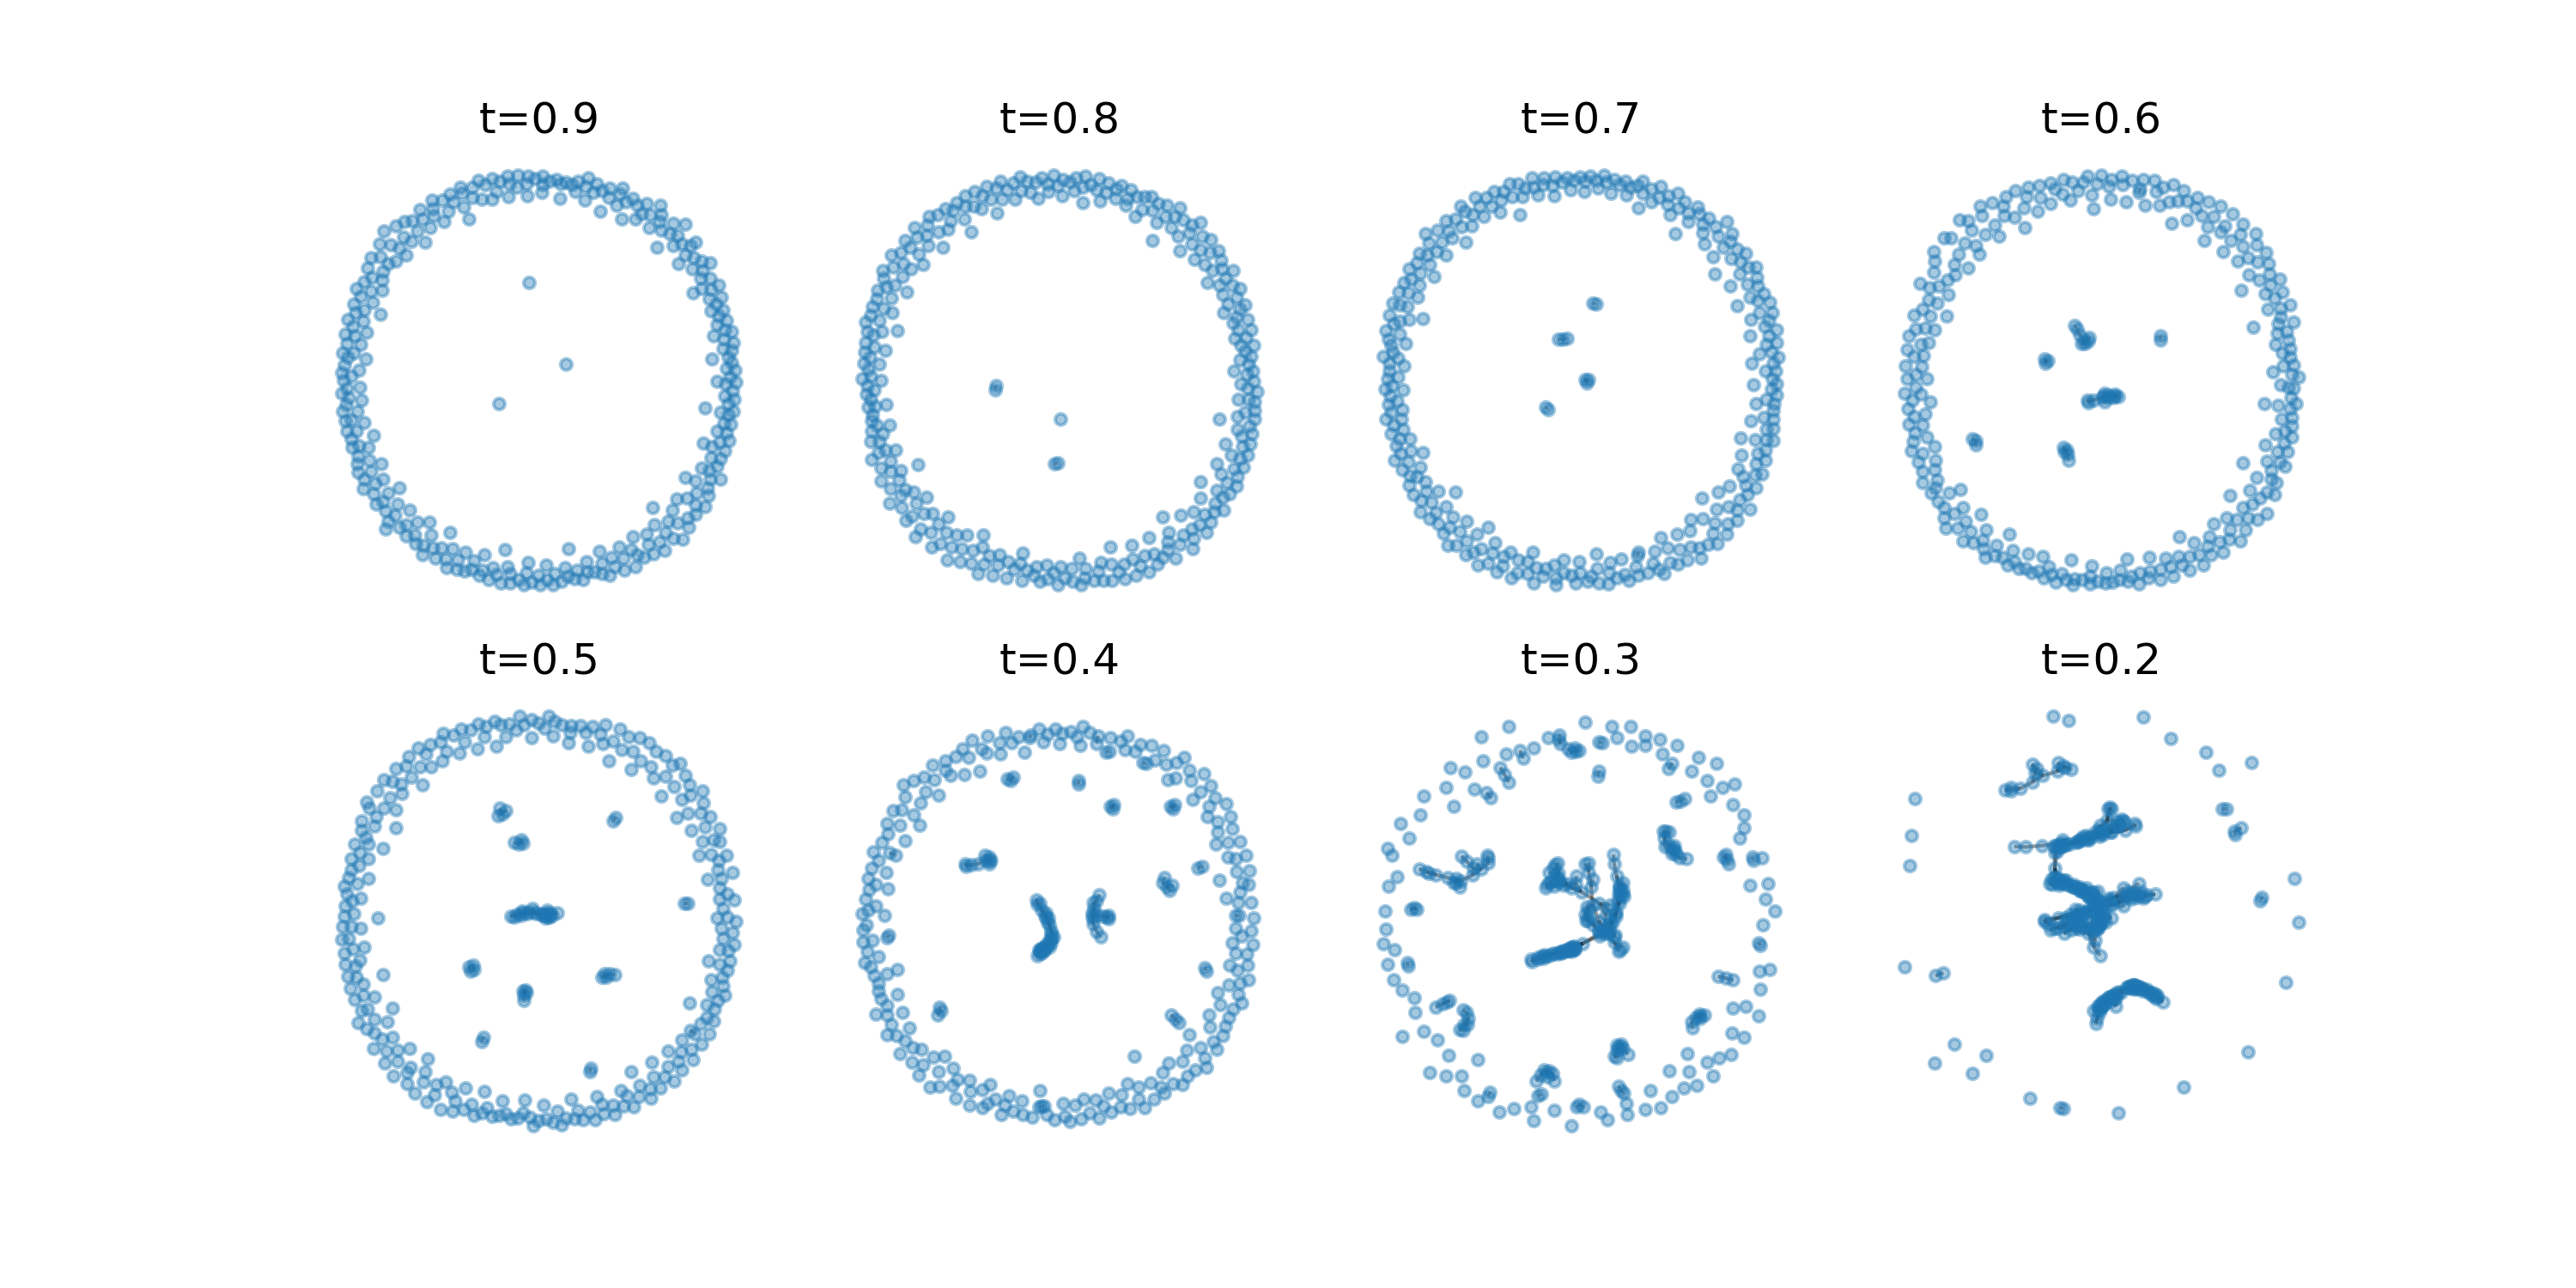
\includegraphics[width=0.75\textwidth]{images/earthquakemultigraphs.png}
\end{figure}
\end{frame}
\begin{frame}{Clique size-Earthquake dataset}
We see that the size of the largest clique increases with a decrease in similarity threshold[greater probability of edge formation]
\begin{figure}
    \centering
    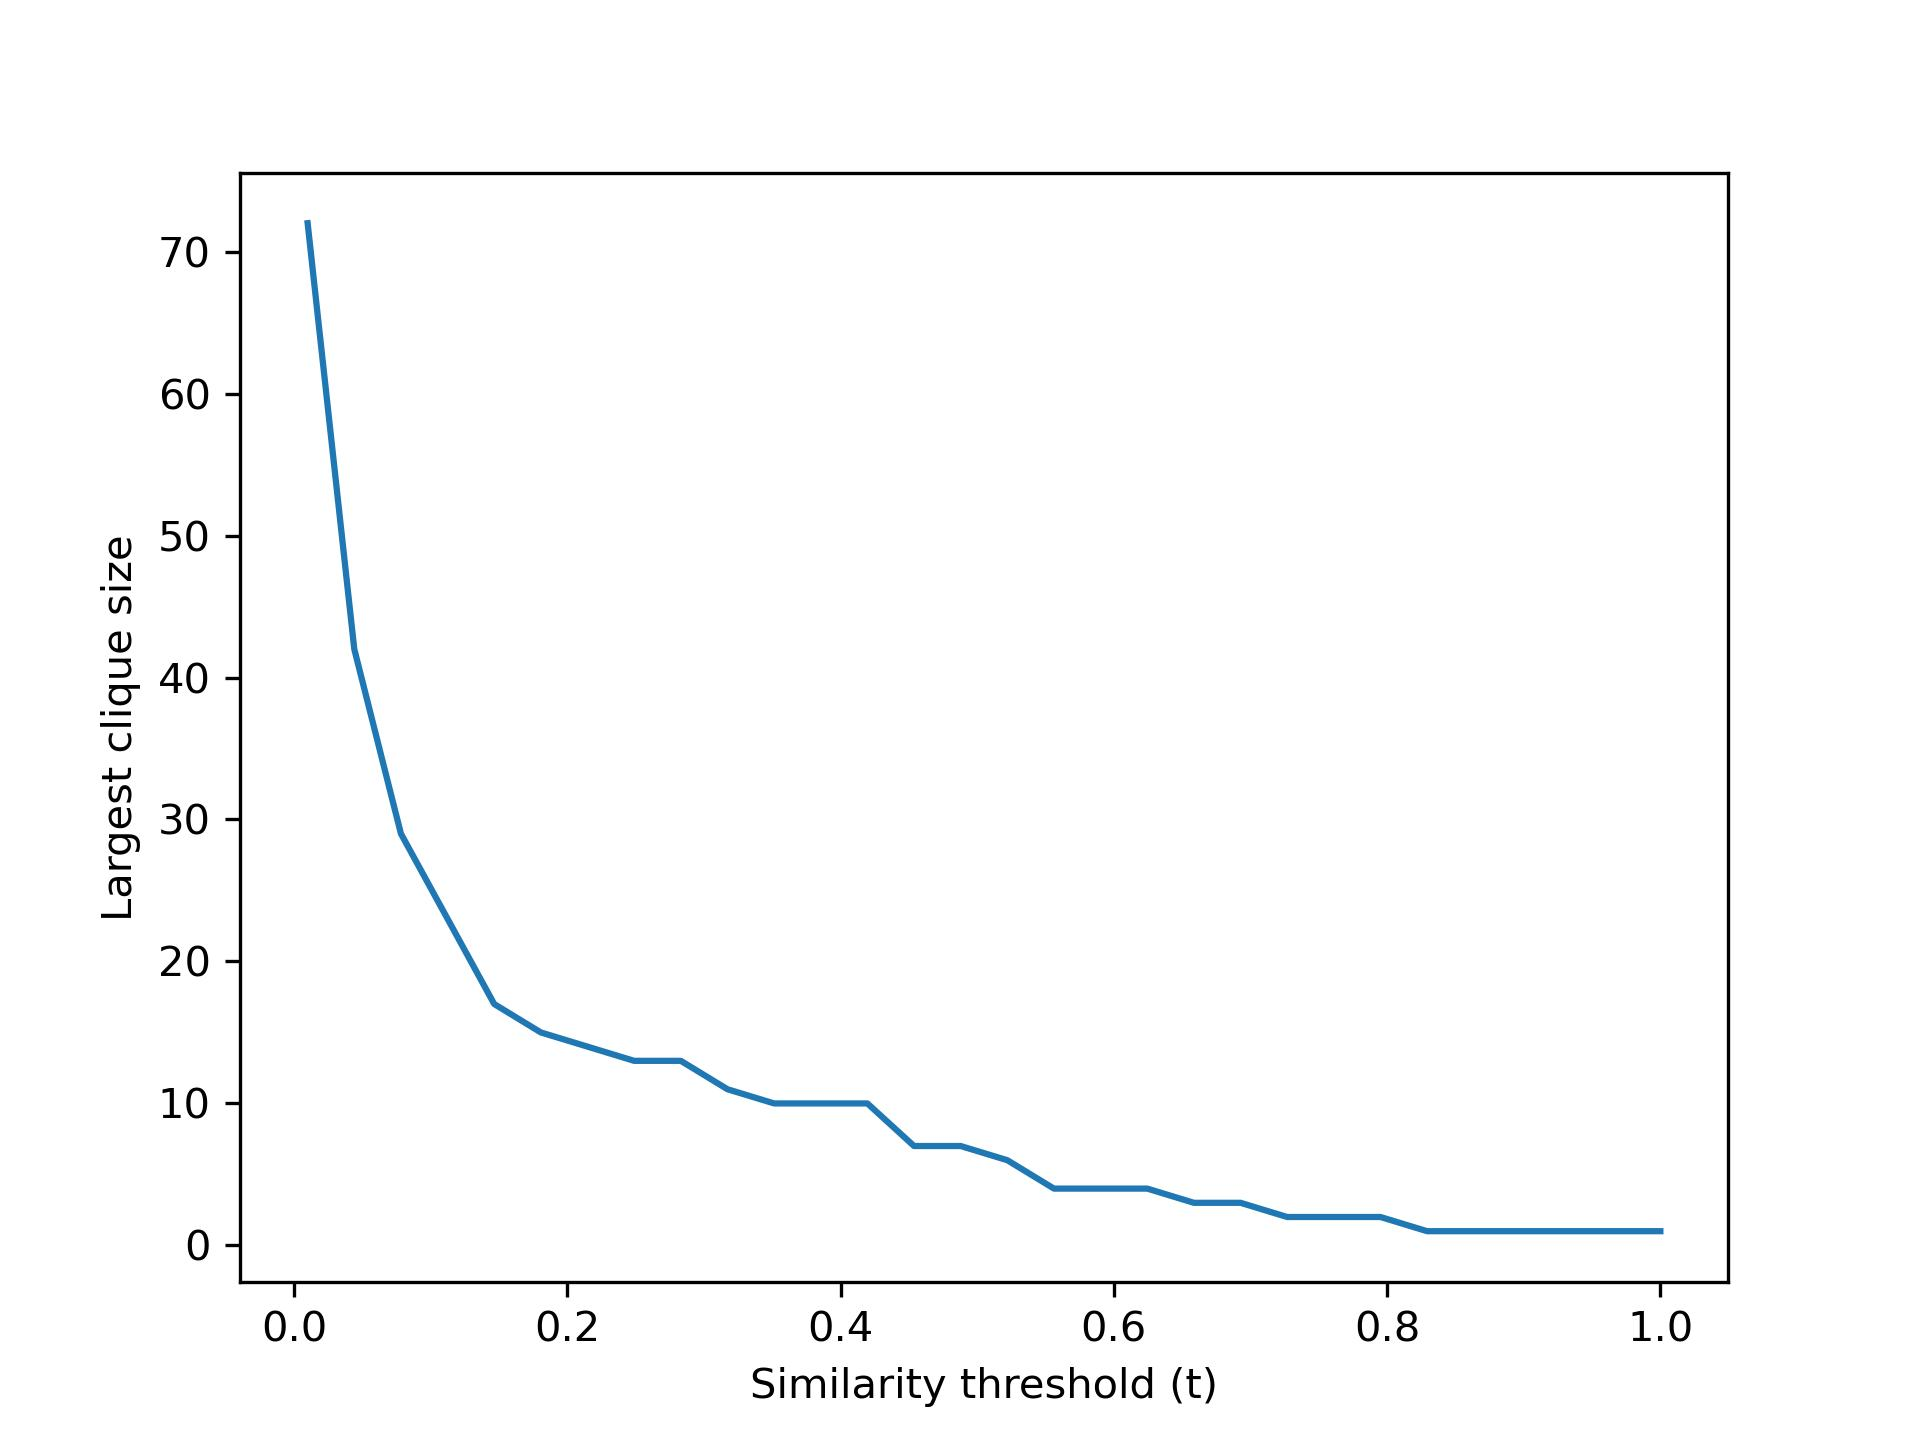
\includegraphics[width=0.5\textwidth]{images/cliquesize.jpg}
\end{figure}
\end{frame}
\begin{frame}{Clustering coifficent and degree distribution-Earthquake dataset}
At $t=0.2$ we get:
\begin{enumerate}[$\bullet$]
    \item The degree of the network is 9.44 with a standard deviation of 6.14.\pause
    \item The clustering coefficient at t = 0.2 to be 0.556961.
\end{enumerate}
\end{frame}
\begin{figure}
    \centering
    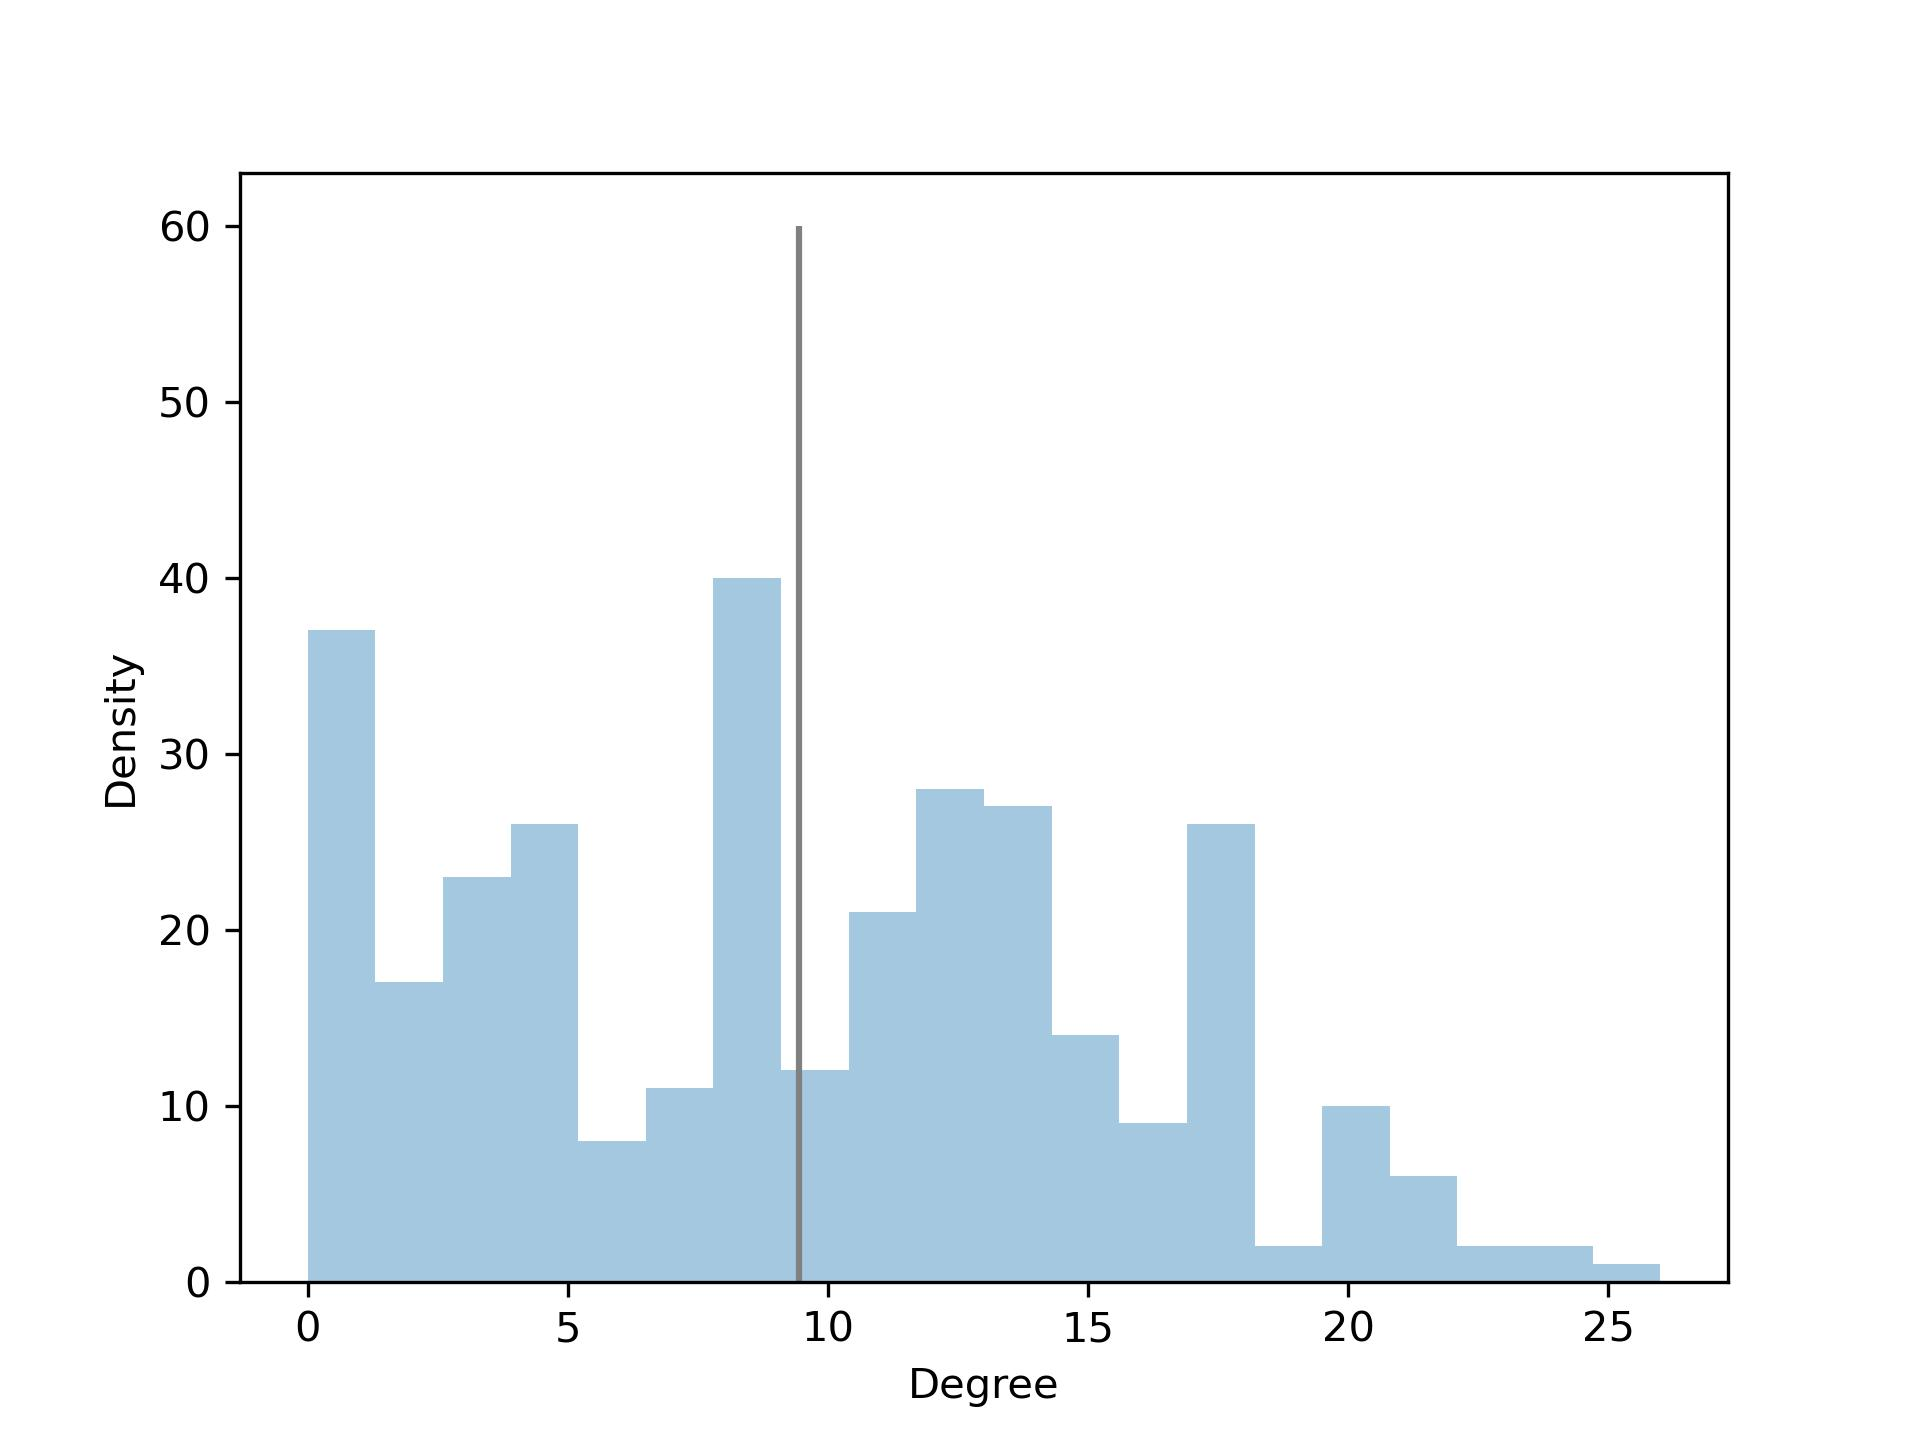
\includegraphics[width=0.5\textwidth]{images/normalizeddegreeDensity(2).jpg}
    \caption{Degree distribution at $t=0.2$}
    \label{fig:my_label}
\end{figure}


\begin{frame}{Manhattan distance-EEG dataset}
    \begin{enumerate}[$\bullet$]
        \item Manhattan distance is the $L^1$ norm\pause
        \item We use this here because there is a large number of observations\pause
        \item We don't need dynamic time wrap because the time series is scynchronised
    \end{enumerate}
\end{frame}



\begin{frame}{Clique formation-EEG dataset}
We consider an edge to form when it crosses the similarity threshold. Therefore as we increase threshold value we see large component formation. \pause We don't include the clique formation images as they are too dense to observe
\end{frame}
\begin{frame}{Clique size-EEG dataset}
We see that the size of the largest clique increases with a decrease in similarity threshold[greater probability of edge formation]
\begin{figure}
    \centering
    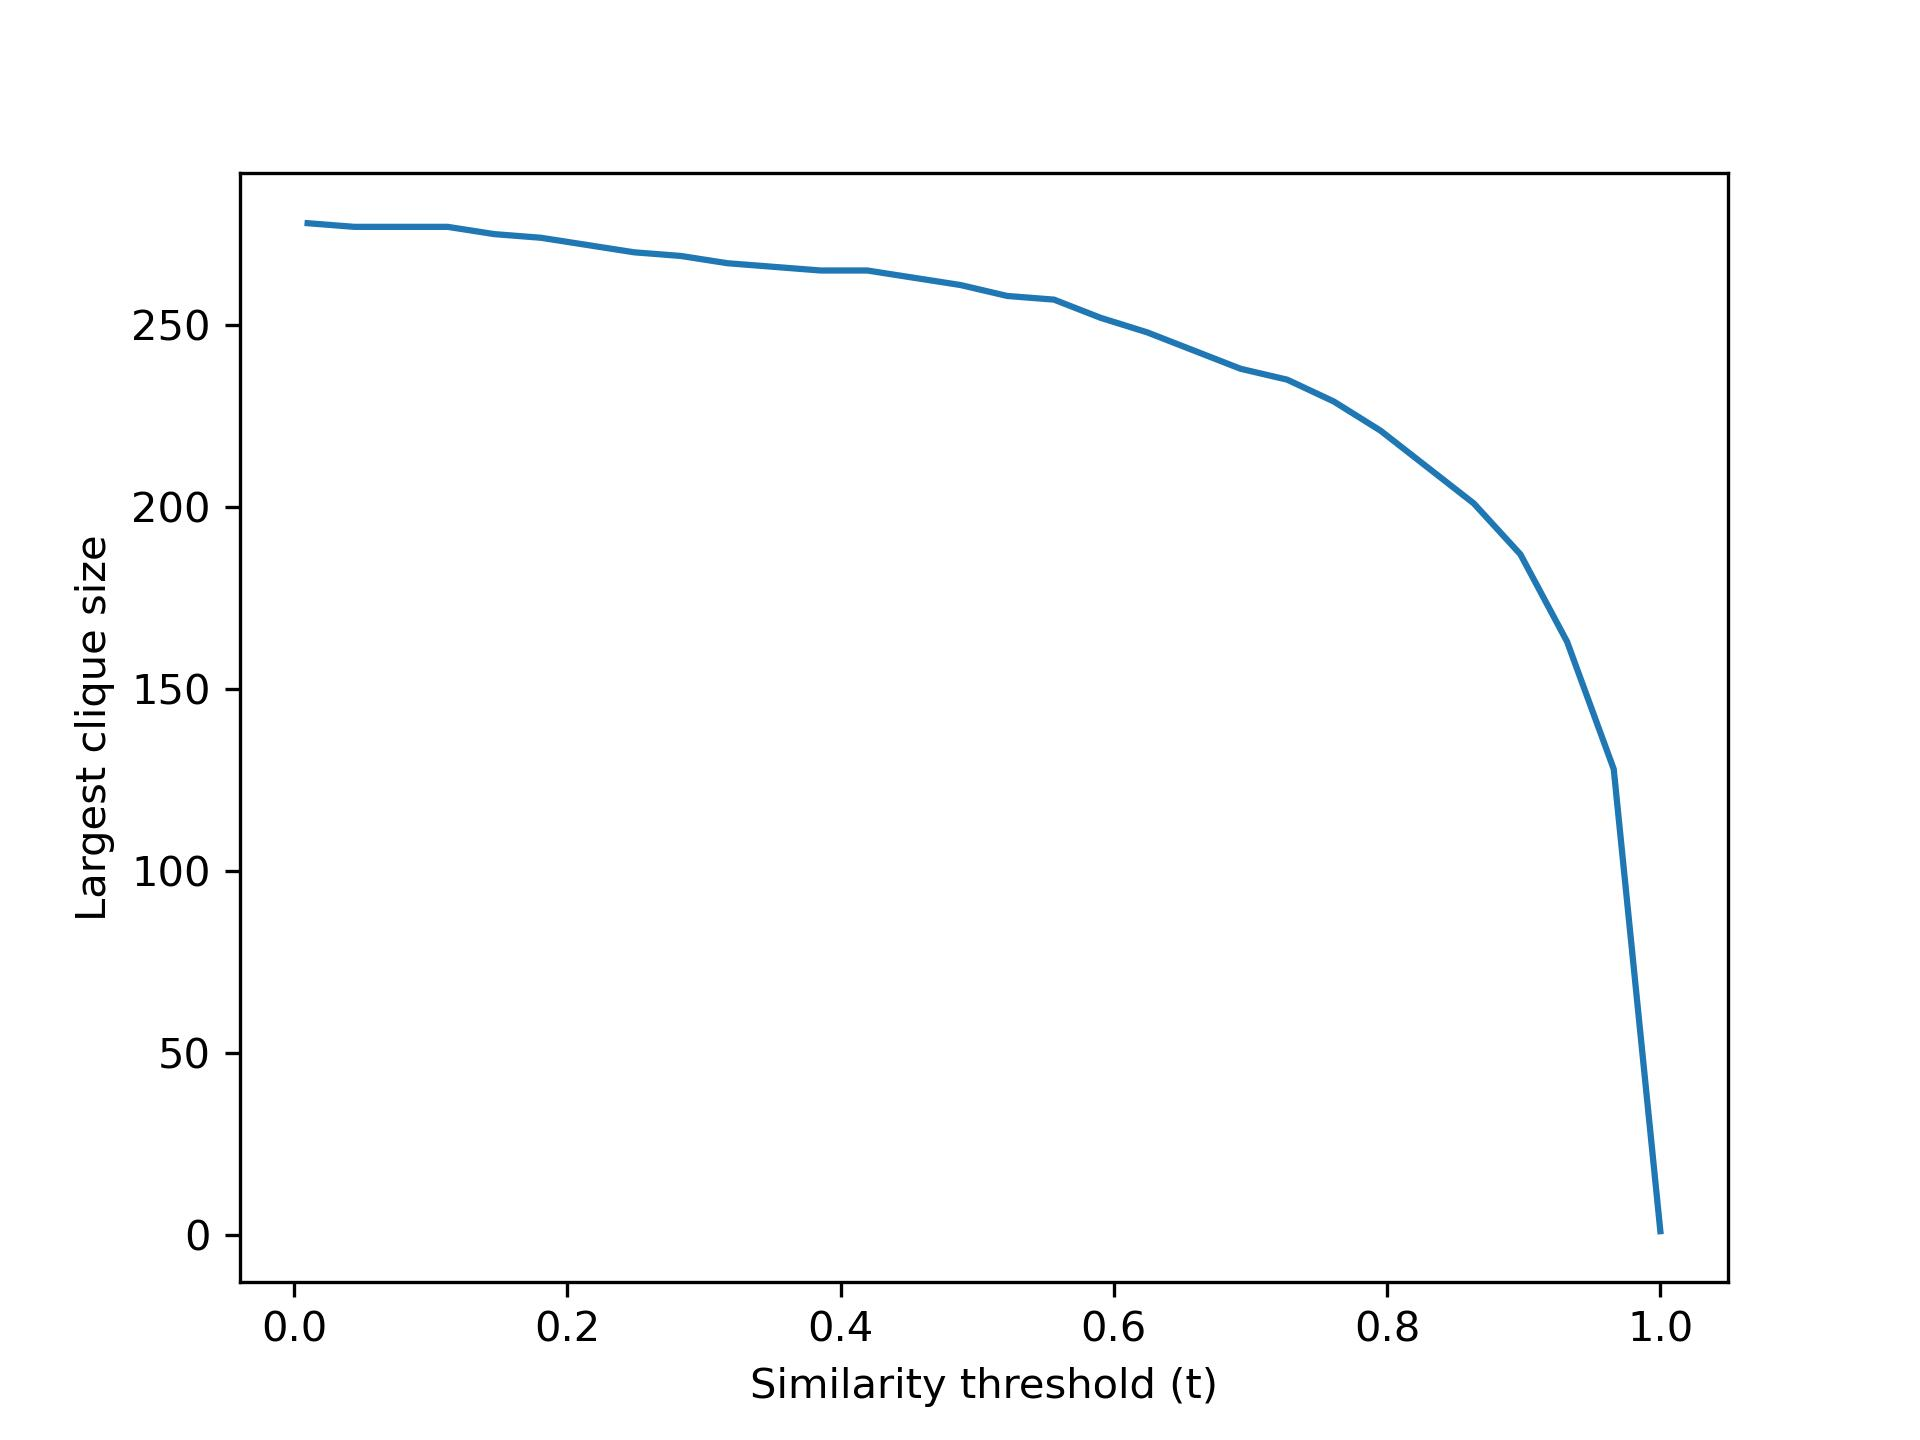
\includegraphics[width=0.5\textwidth]{images/eegcliquesize.jpg}
\end{figure}
\end{frame}
\begin{frame}{Clustering coefficient and degree distribution-EEG dataset}
At $t=0.2$ we get:
\begin{enumerate}[$\bullet$]
    \item The mean degree of the network is 154.36 with a standard deviation of 63.62.\pause
    \item The clustering coefficient at t = 0.93 to be 0.84.
\end{enumerate}
\end{frame}
\begin{figure}
    \centering
    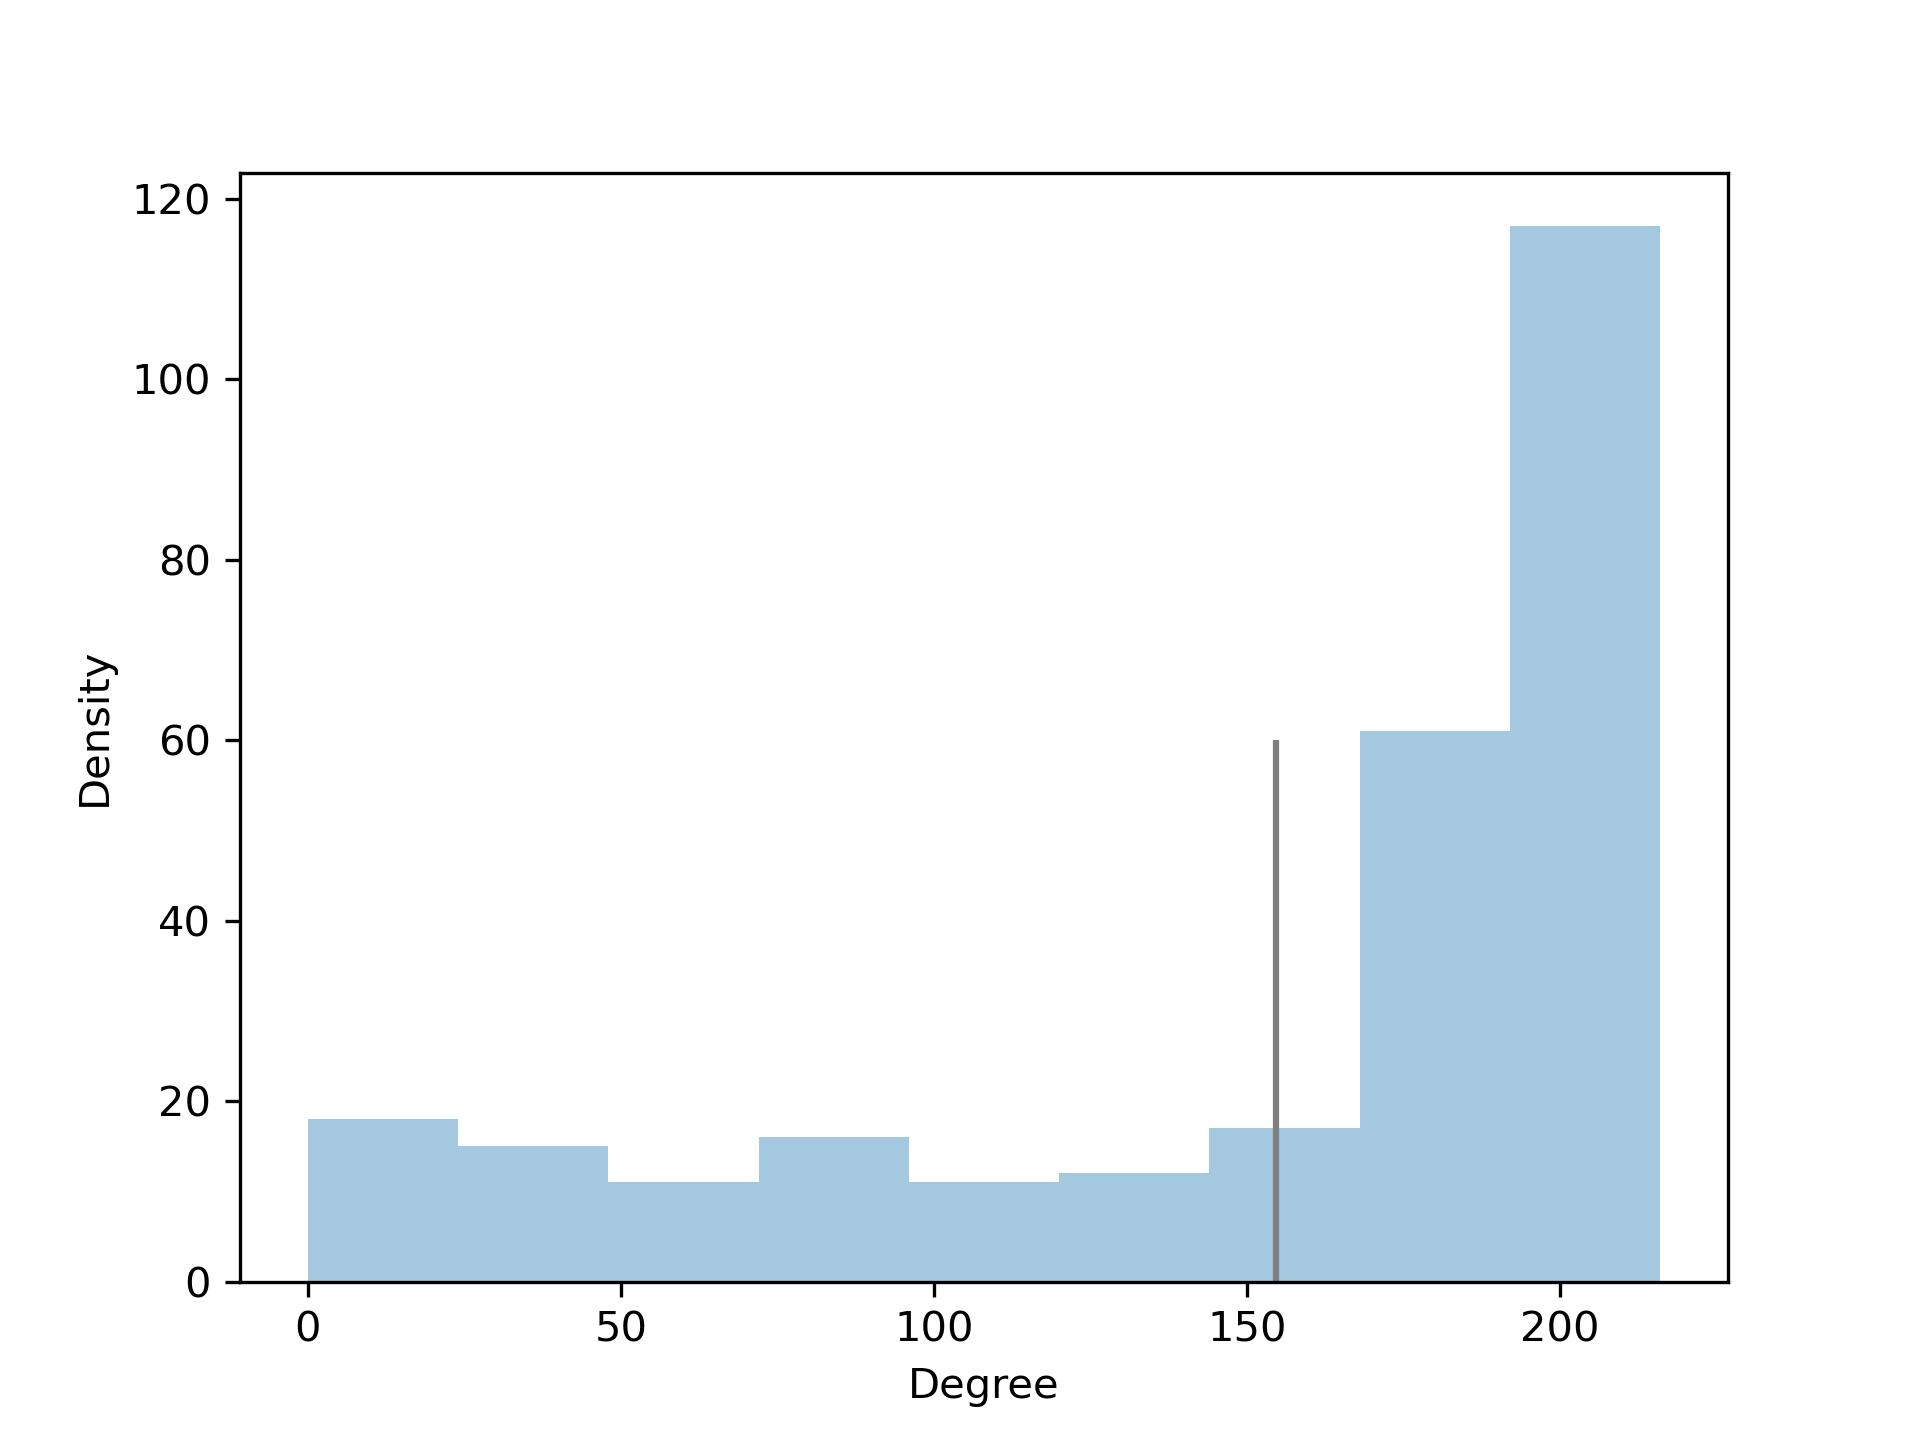
\includegraphics[width=0.5\textwidth]{images/eegnormalizeddegreeDensity.jpg}
    \caption{Degree distribution at $t=0.2$}
    \label{fig:my_label}
\end{figure}




\begin{frame}{Unsupervised Learning}
    Unsupervised learning is a type of machine learning where the goal is to identify patterns or structure in data without the use of labeled output. Clustering is one of the most popular and widely used unsupervised learning techniques. It is a process of grouping similar data points together based on their similarities or distances between them.\pause Here we use K-means as our algorithm of choice.  K-means, work by randomly initializing a specified number of centroids, and then iterating to minimize the distance between each data point and its assigned centroid. The process is repeated until the centroids no longer move or a maximum number of iterations is reached.
\end{frame}

\begin{frame}{Feature seletion and results}
We use the same features as the previous data sets.\pause
We run unsupervised learning and get an accuracy of :
\begin{enumerate}[$\bullet$]
    \item \textbf{EEG Data:} 49\%
    \item  \textbf{Earthquake Data:} 53\%
\end{enumerate}    
\end{frame}

%reference %%edit in 3-reference folder
\begin{frame}{References}
    \nocite{apostol2004mathematical}
    \nocite{fraleigh2003first}
    \bibliographystyle{plain}
    \bibliography{3-reference/ref.bib}
\end{frame}

\end{document}